\section{Apprentissage par Renforcement et Deep Learning}
\label{RL_section}

\textbf{Important}: Ceci ne constitue pas un cours expliquant l'apprentissage par Renforcement. Bien que des notions soient introduites, de nombreux points importants seront ignorés car s'éloignant de la thématique du Deep Learning, de même que la rigueur mathématique\footnote{Nous ne traiterons pas les preuves de convergence des modèles par exemple alors que ça représente un aspect très important des algorithmes d'apprentissage !} qui sera limitée pour faciliter la compréhension générale des idées explicitées.\\

\noindent Les notations peuvent sembler lourdes et les détails mathématiques difficiles à assimiler. Néanmoins, les mathématiques abordées relèvent essentiellement du jeu d'écriture et d'\textit{astuces} à connaître.

\subsection{Approche théorique}
\subsubsection{Généralités}
L'\textit{Apprentissage par Renforcement} est l'une des grandes familles d'apprentissage automatique au même titre que l'apprentissage supervisé et non supervisé par exemple. Cette approche se veut très proche de la méthodologie de l'apprentissage de l'homme basée sur l'expérience et l'analyse des conséquences suite à une action réalisée\footnote{Un enfant apprend de ses chutes jusqu'à réussir à marcher}. Bien que peu répandu en dehors de la Recherche, l'\textit{apprentissage par renforcement} commence à se révéler grâce à sa capacité d'adaptation, sa faible dépendance à des données d'apprentissage pré-fournies et à ses performances. Il est très présent dans le cadre des systèmes autonomes (notamment les véhicules) et de la résolution de jeux (jeux de plateau tels que le Go ou les échecs, jeux vidéo).\\

\noindent Les modèles d'\textit{apprentissage par renforcement} reposent sur les intéractions avec l'environnement et la réponse de cet environnement vis-à-vis de l'action choisie. Ainsi, la problématique peut être formalisée par un agent A, qui à l'instant $t$, au sein d'un environnement, doit choisir une action à réaliser, notée $a_t$ selon l'état $s_t$ dans lequel il se trouve. Après son action, l'environnement fournit une récompense $r_t$ correspondant à la conséquence de cette action sur l'environnement. La récompense peut être positive ou négative selon si la réponse de l'environnement est bénéfique ou non. L'agent se trouve alors dans l'état $s_{t+1}$ et choisit une nouvelle action à réaliser (ou s'arrête selon le cas). La Figure \ref{genrefpic} résume cette problématique. L'objectif de cet apprentissage est donc de définir un modèle capable de maximiser les gains de récompenses.

\paragraph{L'environnement}
L'environnement représente le milieu où évolue l'agent. Il peut présenter différentes spécificités:
\begin{itemize}
    \item \textbf{Déterministe/Stochastique}: Lors d'une action $a_t$ à partir d'un état $s_t$, l'agent arrive dans l'état $s_{t+1}$. L'environnement est défini par un espace d'états S fini ou non et d'un espace d'actions possibles A. Il est \textit{déterministe} si:
    $$\forall a_t,s_t \in (A_{s_t},S), \  \exists \ s_{t+1} \in S, \ P(s_{t+1} \ | \ a_t,s_t)=1$$
    Sinon, il est considéré comme \textit{stochastique}. Un environnement \textit{déterministe} est défini par un environnement qui, pour tout stimuli de même nature, réagit de la même manière à partir d'un état donné. Par exemple, si on suppose le jeu Mario, lorsqu'on exécute l'action "sauter", Mario va sauter à chaque fois (si l'état à partir duquel l'action est faite le permet). Au contraire, un environnement est stochastique si:
    $$\forall a_t,s_t \in (A_{s_t},S), \ \exists \ s_{t+1} \in S, \ P(s_{t+1} \ | \ a_t,s_t)<1$$
    Cette particularité associe un facteur probabiliste à l'environnement. Ainsi, suite à une action et un état donnés, l'état suivant est déterminé selon une distribution probabiliste. Supposons une voiture, l'action d'accélérer peut réaliser l'accélération ou, dans d'autres cas, ne pas fonctionner en cas d'une panne par exemple.

    \item \textbf{Observable ou Partiellement Observable}: L'environnement est défini comme observable lorsque l'ensemble des états qui le forme sont pleinement définis et connaissables. Au contraire, l'environnement est défini comme partiellement observable lorsque les états ne sont pas ou partiellement connaissables et que l'acteur n'a accès qu'à des observations. Ainsi, un environnement partiellement observable est défini par une fonction de transitions entre les observations (qui définit la probabilité d'observer un phénomène à partir d'une action dans un état donné) et d'une fonction de perception liant observations et état (qui définit la probabilité d'avoir une observation dans un état). Ainsi, supposant, S, ensemble des états, A, ensemble des actions et Z, ensemble des observations, la fonction de transition entre observations est définie par:
    $$(s_t,a_t,z_{t+1}) \in (S,A_{s_t},Z_{s_t}), \ T(s_t,a_t,z_{t+1})=P(z_{t+1} \ | \ s_t, a_t)$$
    La fonction de perception, noté $\varphi$, est définie par:
    $$(s_t,z_t) \in (S,Z_{s_t}), \ \varphi(s,z)=P(z_t \ | \ s_t)$$

    \item \textbf{Discret/Continu}: Dans la configuration d'un environnement discret, le temps évolue de manière séquentielle. Ainsi, la fonction temps est définie par un pas discret soit de t à t+1. Dans le cas continue, le temps évolue de manière continue soit de t à t+$\Delta t$ avec $\Delta t$ infiniment petit. De ce fait, un état n'évolue pas de manière discrète mais varie continuellement selon une quantité $\frac{ds}{dt}$ qui peut être comparée à une vitesse de variation d'état.

    \item \textbf{Connu/Inconnu}: L'environnement peut être inconnu de l'acteur. Ainsi, il peut ne pas connaître les récompenses obtenues, les fonctions de transitions voire même les états eux-mêmes. Au contraire, il peut aussi évoluer dans un environnement clairement établi et défini en amont. Par exemple, calculer l'itinéraire d'un trajet peut être associé à un environnement connu. Apprendre à un automate à marcher "par lui-même" est un problème à environnement inconnu car l'automate ne connaît pas l'impact de ses actions ni-même l'étendu des possibilités des différentes postures qu'il peut visiter durant son apprentissage.

    \item \textbf{Stationnaire/Non Stationnaire}: L'environnement peut varier au cours du temps. De ce fait, les récompenses et les fonctions de transitions peuvent ne pas être constantes. Un environnement variable implique un apprentissage permanente et évolutif de l'acteur. Si l'évolution de l'environnement suit un processus aléatoire, l'apprentissage ne peut être réalisé pleinement si ce n'est l'adaptation de l'acteur à son nouveau milieu. Si l'évolution est aléatoire et permanente, l'acteur ne peut apprendre. Comment peut-on jouer à un jeu dont les règles évoluent tout le temps de manière aléatoire ?

    \item \textbf{Fini/Infini}: L'environnement peut posséder un nombre fini d'états comme pour un jeu de plateau par exemple. Au contraire, il peut aussi avoir un nombre infini d'états. Un problème avec un nombre infini d'états est souvent associé à un problème à temps continu qui, du fait du nombre infiniment grand d'états, est jugé à environnement infini.
\end{itemize}

\begin{figure}
\centering
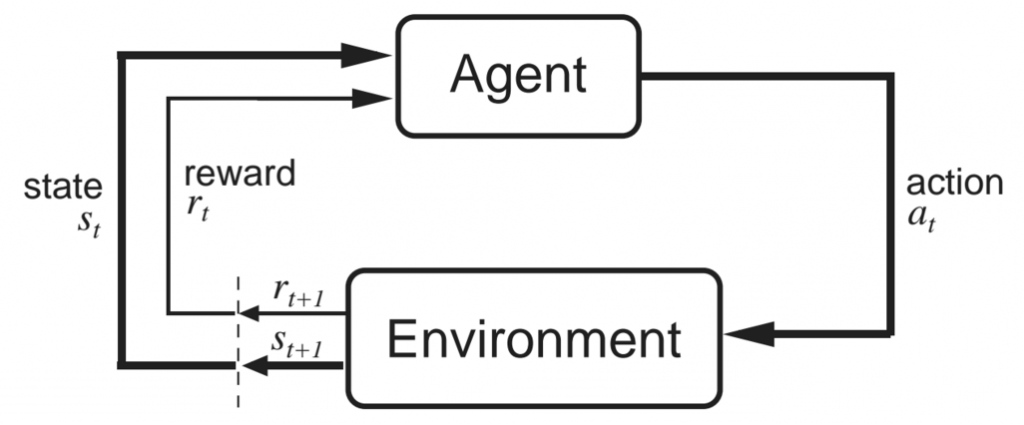
\includegraphics[scale=0.3]{./tex/reinforcement-learning/genrenf.png}
\caption{Graphique séquentiel de l'approche par renforcement}
\label{genrefpic}
\end{figure}

\paragraph{Formalisation du problème}
Supposons un environnement stationnaire entièrement observable où le temps est discret. Le problème peut être formalisé par un \textbf{problème de décision de Markov} (PDM). Ce problème est défini par le quadruplet (S,A,P,R) défini tel que:
\begin{itemize}
    \item \textbf{S}: ensemble d'états \textbf{finis}
    \item \textbf{A}: ensemble d'actions fini tel que A(s) est associé à l'ensemble des actions réalisables à l'état s\footnote{Il se peut qu'un sous-ensemble uniquement de A soit réalisable dans un état s de S}
    \item \textbf{T}: Fonction de transition qui explicite la dynamique de transition entre états pour une action donnée:
    $$(s,a,s') \in (S,A,S) \rightarrow P(s,a,s')=Pr(s_{t+1}=s' \ | \ a_t=a,s_t=s)$$
    \item \textbf{R}: Fonction de récompenses sur $\mathcal{R}$ qui explicite l'espérance (valeur moyenne) des récompenses renvoyées par l'environnement associées à chaque changement d'état. Elle est définie par:
    $$(s,a,s') \in (S,A,S) \rightarrow R(s,a,s')=E(r_t \ | \ a_t=a,s_t=s,s_{t+1}=s')$$
\end{itemize}

\noindent Le problème est à \textit{horizon fini} si il existe un (des) état(s) dits \textit{final(aux)}, i.e provoque la fin de l'expérience. Par exemple, la fin d'une partie d'un jeu. Cette particularité permet ainsi la réalisation de plusieurs expériences distincts nommées \textit{itérations} car le problème est à durée finie. Au contraire, le problème peut être à \textit{horizon infini}. Il ne possède donc pas d'état(s) final(aux) et de ce fait, il n'y a qu'une expérience (à durée non finie). Par exemple, la survie d'un robot en mission\footnote{On peut, selon le point de vue, considérer la panne d'énergie ou l'usure du robot comme un état final si il implique son arrêt total}.\\

\noindent \textbf{Important}: On considère que l'état actuel ne dépend \textbf{QUE} de l'état précédent et de l'action qui y a été réalisée. Ainsi, la fonction de transition ne considère que l'action et l'état précédents pour choisir l'état actuel. Ceci est une hypothèse très forte qui suppose qu'une situation à l'instant t dépend exclusivement de la situation à l'instant t-1. Ceci est généralement faux dans les faits ! Cette hypothèse est appelée l'\textbf{hypothèse de Markov}.\\

\noindent Lorsqu'on ne considère que la situation précédente pour choisir l'état actuel, on décrit un problème de Markov \textbf{d'ordre 1}. Si on considère la situation t-1 et t-2, nous obtenons un problème de Markov \textbf{d'ordre 2}. Par convention un PDM est défini si l'hypothèse de Markov d'ordre 1 est définie. Néanmoins, tout problème de Markov d'ordre n peut être ramené à un problème de Markov d'ordre 1 en augmentant le nombre d'états.

\paragraph{Définitions fondamentales}
L'objectif de l'acteur est de maximiser \footnote{Ou de minimiser selon la formulation de la problématique} les récompenses obtenues durant les intéractions avec l'environnement. Notons $r_t$, la récompense obtenue par l'acteur à l'instant t. Le \textit{Retour} définit la somme des récompenses obtenues par l'acteur à partir de l'instant t. Nous avons donc:
$$ R_t=\sum_{k=0}\gamma^k r_{t+k}$$
Avec $\gamma \in [0,1]$. Ce facteur est appelé \textit{facteur de dépréciation}. Il permet de pondérer l'importance des récompenses obtenues selon la proximité temporelle. Si $\gamma=1$, toutes les récompenses sont considérées avec la même intensité. Le système a donc un raisonnement à très long terme. Au contraire, si $\gamma \rightarrow 0$, le système ne considère que les récompenses proches et n'a pas de vision à long terme. Ce coefficient est très important en cas \textit{d'horizon infini} car, étant donné l'absence d'état final, l'expérience n'a "pas de fin". Il est donc nécessaire de borner la somme par l'ajout de ce critère qui délimite la vision à long terme.\\

\noindent La \textit{politique} représente la capacité de décision de l'agent. Elle définit l'action qui est choisie selon les critères qu'elle considère. Ainsi, nous la représentons telle que:
$$ (s,a) \rightarrow (S,A), \  \pi(s,a)=P(a_t=a|s_t=s)$$

\noindent La politique est donc caractérisée par la probabilité de réaliser une action spécifique dans un état s de S. La définition précédente définit une politique \textit{stochastique}. Selon les spécificités voulues pour le modèle, il est possible de désirer une politique \textit{déterministe} où chaque état est associé à une action unique (probabilité de 1\footnote{la politique choisit une action unique mais l'environnement peut être stochastique et faire en sorte que l'agent ne finisse pas nécessairement dans l'état choisi par la politique. Il faut bien différencier l'aspect stochastique de la politique et de l'environnement}). De ce fait, la politique suit la définition:
$$ s \rightarrow S, \ \pi(s)=a$$

\noindent Un état possède une valeur qui représente sa qualité\footnote{Par convention, plus la valeur est élevée, plus l'état est qualitatif donc présentant un intérêt à l'atteindre par l'agent}. Cette valeur est liée à la politique et variable dès lors que la politique évolue. Elle est définie par l'espérance des récompenses cumulatives à partir de l'état ciblé peu importe les actions réalisées par la suite. Ainsi, pour un état $s \in S$ et une politique $\pi$, nous avons:
$$V^\pi(s)=E(R_t|s_t=s)$$

\noindent Alors que V évalue la qualité d'un état peu importe les actions réalisées, Q définit une valeur d'un couple \textit{état-action} pour une politique $\pi$ donnée. Q évalue donc la qualité d'un état en considérant l'action qui a mené à cet état, au contraire de V qui l'ignore. Nous avons donc:
$$Q^\pi(s,a)=E(R_t|s_t=s, a_t=a)$$

\paragraph{L'équation fondatrice: l'équation de Bellman}
Nous avons vu que:
$$ R_t=\sum_{k=0}\gamma^k r_{t+k}$$
$$V^\pi(s)=E(R_t|s_t=s)$$

\noindent Par un jeu d'écriture, nous pouvons donc redéfinir $V^\pi$.
\begin{align}
   V^\pi(s) &= E(R_t|s_t=s) \\
   & = E(\sum_{k=0}\gamma^k r_{t+k}|s_t=s)\\
   & = E(r_t + \sum_{k=1}\gamma^k r_{t+k}|s_t=s)\\
   & = E(r_t + \gamma \sum_{k=1}\gamma^{k-1} r_{t+k}|s_t=s)\\
   & = E(r_t) + \gamma E(\sum_{k=1}\gamma^{k-1} r_{t+k}|s_t=s)
\end{align}

\noindent Or, nous pouvons constater que:
$$V^\pi(s_{t+1})=E(\sum_{k=1}\gamma^{k-1} r_{t+k}|s_t=s)$$

\noindent $E(r_t)$ présente une difficulté car l'espérance doit considérer toutes les situations possibles. Il est donc nécessaire de tenir de compte de l'aspect \textit{stochastique} de la fonction de transition et de la politique. Dans une configuration \textit{déterministe}, l'équation en sera qu'un cas particulier. Supposons $R(s_t,a_t,s_{t+1})$\footnote{Valeur issue de la fonction récompense définie par le PDM}, espérance de la récompense obtenue en passant de l'état $s_t$ à $s_{t+1}$ par l'action $a_t$. Dans un premier temps, nous considérerons l'environnement et la politique comme \textit{déterministes}. Ainsi, chaque action garantit d'atteindre l'état-cible et la politique choisit toujours la même action pour un état donné. Nous obtenons donc:
$$E(r_t)=R(s_t,a_t,s_{t+1})$$

\noindent Supposons l'environnement comme stochastique. L'état-cible n'est donc plus garanti d'être atteint mais relève d'une considération probabiliste. De ce fait, la valeur de récompense associée à l'état actuel repose sur la somme des différentes valeur de récompenses obtenues en atteignant les différents états de l'environnement possibles. Nous avons donc:
$$E(r_t)=\sum_{s_{t+1} \ \in \  S} P(s_t,a_t,s_{t+1})R(s_t,a_t,s_{t+1})$$

\noindent Avec la même approche, supposons une politique et un environnement stochastiques. Nous obtenons alors:
$$E(r_t)=\sum_{a_t \ \in A(s)} \pi(s_t,a_t) \sum_{s_{t+1} \ \in \  S} P(s_t,a_t,s_{t+1})R(s_t,a_t,s_{t+1})$$

\noindent Par un calcul analogue, nous pouvons donc redéfinir $V^\pi(x)$. Cette équation, nommée \textbf{équation de Bellman}, est au coeur de la théorie de l'apprentissage par renforcement et constitue le socle théorique fondamental de cette famille d'algorithme. Elle est définie par:
$$V^\pi(s_t)=\sum_{a_t \ \in A(s)} \pi(s_t,a_t) \sum_{s_{t+1} \ \in \  S} P(s_t,a_t,s_{t+1})(R(s_t,a_t,s_{t+1}) + \gamma V^\pi(s_{t+1}))$$

\noindent L'objectif du modèle est d'obtenir la politique optimale qui maximise les valeurs d'états. Nous noterons la fonction valeur de la politique optimale, $V^*(s)$. Elle constitue l'\textbf{équation d'optimalité de Bellman}.
$$V^*(s)=max_\pi V^\pi(s)=\underset{a \ \in \ A(s)}{max} \sum_{s_{t+1} \ \in \  S} P(s_t,a_t,s_{t+1})R(s_t,a_t,s_{t+1}) $$
\paragraph{Model-Free et Model-Based}
En connaissant l'ensemble des éléments du MDP, il est "aisé" de définir une solution avant d'interagir avec l'environnement. On peut donc considérer ce problème comme un problème de \textit{planification} usant d'algorithmes de \textit{programmation dynamique}\footnote{Nous ne détaillerons pas ces algorithmes dans ce cours}. Dans les faits, l'environnement est rarement parfaitement connu, i.e la fonction de récompenses et de transitions sont inconnues. L'agent doit donc être capable d'évoluer sans connaissance préalables de l'environnement où il se trouve. Pour cela, il existe deux approches d'apprentissage: \textbf{Model-Free} et \textbf{Model-Based}.\\

\noindent \textbf{Model-Based} repose sur l'idée que l'agent doit apprendre un modèle qui approxime les caractéristiques de l'environnement pour définir une politique optimale. A partir de son approximation, il est capable de définir le comportement optimal à suivre pour réaliser son objectif. Ainsi, si l'agent est dans l'état $s_t$, qu'il réalise l'action $a_t$ et qu'il atteint l'état $s_{t+1}$ avec une récompense $r_{t+1}$, alors le modèle cherchera à améliorer son estimation de $P(s_{t+1}|s_t,a_t)$ et de $R(s_t,a_t)$ à travers les valeurs de V. Le modèle apprendra donc les conséquences de la réalisation d'une action dans un état donné. A partir des conséquences connues, le modèle définira la politique la plus performante.\\

\noindent \textbf{Model-Free} s'émancipe de l'approximation du modèle pour définir une politique. Il n'y a donc pas d'approximation de l'environnement, i.e de la fonction de transitions et de récompenses. Le modèle cherche donc à apprendre directement la politique à suivre, i.e quand choisir telle action. L'algorithme \textit{Q-Learning}\cite{qlearning} est l'algorithme de référence pour ce type d'approche.

\paragraph{Différence temporelle}
Une des principales faiblesses des premières approches par apprentissage par renforcement (sans connaissances explicites du PDM) était la nécessité de devoir finir une itération pour mettre à jour le modèle (par exemple, la méthode de Monte-Carlo). Ce type d'approche demande du temps et surtout, est inefficace dans le cadre d'un environnement à \textit{horizon infini}\footnote{Un environnement sans état final donc sans "fin" d'expérience explicite}\footnote{Ceci n'est pas complètement vrai. Il existe des "astuces" pour ignorer ce type de contraintes mais nous ne les considérerons pas}. Afin de palier à cette faiblesse, la notion de \textit{différence temporelle} a été introduite par Sutton dans son article de recherche \cite{difftemp}.\\

\noindent Nous avons vu que que pour une politique $\pi$ donnée, nous avons:
$$V^\pi (s_t)=r_t+\gamma V^\pi (s_{t+1})$$

\noindent Par un simple jeu d'écriture, nous obtenons:
$$\underbrace{r_t+\gamma V^\pi (s_{t+1})}_{Temporal \ Difference}- \ V^\pi (s_t)=0$$

\noindent Durant l'apprentissage, cette égalité n'est pas vérifiée. Si la valeur actuelle de $V^\pi (s_t)$ est trop élevée, la valeur TD sera négative et positive dans le cas contraire. Cette valeur permet donc d'orienter l'évolution de $V^\pi (s_t)$. La correction se présente sous la forme:
$$V^\pi_{t+1}(s_{t}) \rightarrow V_t^\pi (s_t)+\alpha (r_t+\gamma V_t^\pi (s_{t+1})-V_t^\pi (s_t))$$

\noindent Avec $\alpha \in [0,1]$. $\alpha$ est associé à un taux d'apprentissage. Il est pertinent pour se protéger de la condition de stochasticité de l'environnement. En effet, si il est déterministe, nous sommes "sûr" de la modification à réaliser sur V. De ce fait, nous pouvons exploiter un taux égal à 1. Au contraire, si l'environnement est stochastique, les modifications sont incertaines car dépendantes de la distribution des états. Initialement, nous considérerons une valeur proche de 1 car la distribution est inconnue. Cela permet des mises à jour grossières et importantes (souvent très oscillantes) le temps d'estimer les distributions convenablement. Avec le temps, le taux tendra vers 0 car les distributions seront bien estimées via les valeurs de V et pour permettre une bonne convergence du modèle. Pour une approche par défaut, il est commun de définir $\alpha$ comme une fonction dépendante de l'état considérée tel que:
$$\alpha(s)=\frac{1}{1+nombre \ de \ visite \ de \ s}$$

\noindent \textit{Temporal difference} est utilisée au sein d'un algorithme nommé TD(0) qui exploite sa capacité de correction pour évaluer les valeurs d'états pour une politique donnée (model-based). Il est défini sur la Figure \ref{tdalgo}.

\begin{figure}
    \centering
    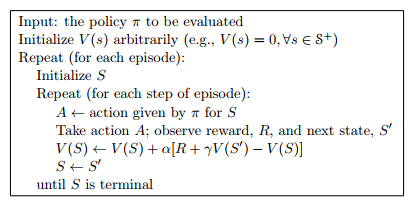
\includegraphics[scale=0.4]{./tex/reinforcement-learning/tdalgo.png}
    \caption{Algorithme du TD(0)}
    \label{tdalgo}
\end{figure}

\paragraph{Un standard: l'algorithme Q-Learning}
TD(0) évalue une politique mais ne permet pas de la mettre à jour. Il est donc nécessaire de proposer une autre méthode capable de proposer une politique améliorée. Il est possible d'exploiter des méthodes "standards"\footnote{non traitées dans ce cours} pour exploiter le résultat de TD(0) ou d'utiliser un autre algorithme qui permet d'apprendre une politique de manière autonome comme l'algorithme \textit{Q-Learning}.\\

\noindent Cette algorithme repose sur la même approche que TD(0) sauf qu'il exploite les valeurs Q et non V. De ce fait, il considère les couples(état,action) et non juste les états. Son comportement est donc spécifique aux actions et non cumulatif comme le fait TD(0). L'algorithme est détaillé sur la Figure \ref{qalgo}.\\

\noindent Deux spécificités importantes sont à approfondir. La première est l'utilisation de $max(Q(s_{t+1},a_{t+1})$. Par conséquent, le modèle exploitera toujours la valeur de Q associée à la meilleure action à faire dans l'état t+1, indépendamment de l'action qui sera véritablement réalisée (la meilleure action n'est pas forcément celle qui est réalisée !) dans cet état. On caractérise les algorithmes usant de ce type d'approche comme  des algorithmes \textbf{off-policy}. Un autre algorithme, nommé \textit{SARSA}\cite{sarsa}, exploite la même approche que \textit{Q-Learning} à la différence que \textit{SARSA} n'exploite pas la valeur max mais la valeur effectivement choisie par le modèle. C'est ainsi un algorithme dit \textbf{on-policy}.\\

\noindent La différence effective entre les deux algorithmes est "l'audace" de l'agent. En effet, Q-Learning n'exploite que les meilleures valeurs indépendamment des actions réelles effectuées. De ce fait, Q-Learning ne tient pas compte de situations potentiellement néfastes pour l'agent car la mise à jour des valeurs de Q ne considère pas l'action réellement effectuée. Au contraire, SARSA considère l'ensemble des situations que l'agent visite et se met à jour en adéquation avec les situations "dangereuses" observées. Ce modèle sera donc beaucoup plus prévenant et moins audacieux qu'un agent sous Q-Learning. Pour imager, supposons qu'un individu souhaite aller d'un point A à un point B où ces deux points sont au bord d'une falaise. L'agent sous Q-Learning se déplacera le long du bord jusqu'à arriver à destination. En effet, c'est le chemin le "plus court" et efficace. Cependant, il ne tient pas compte du risque (peu probable mais réel) de chute possible. Au contraire, l'agent sous SARSA s'éloignera légèrement du bord, augmentant la distance parcourant mais évitant le piège de la chute. Q-Learning favorise l'efficacité par rapport au risque alors que SARSA réalise un compromis entre les deux. Il n'y a pas de meilleure approche. Tout dépend de la problématique à traiter et du contexte de l'agent.\\

\noindent La seconde spécificité à comprendre est la politique choisie par Q-Learning (ou pour SARSA). Avant de présenter ces politiques, il est nécessaire d'introduire la notion de \textbf{compromis exploration/exploitation}.\\

\noindent Pour obtenir une bonne compréhension de l'environnement, il est nécessaire de l'explorer et de le visiter. Cette étape est appelée \textbf{exploration}. Lorsque l'environnement est assimilé et connu, il n'est plus pertinent de visiter mais au contraire, il est nécessaire d'exploiter la connaissance obtenue. Cette étape est nommée \textbf{exploitation}. Un compromis entre ces deux comportements est au coeur de l'apprentissage par renforcement car c'est l'exploration qui permet de détecter les comportements les plus bénéfiques mais uniquement l'exploitation est capable de les exploiter. La difficulté est donc de comprendre à quel moment l'agent a suffisamment exploré pour pouvoir exploiter ses connaissances.\\

\noindent Différentes politiques peuvent être exploitées dont les plus répandues sont:
\begin{itemize}

    \item Approche indépendante de la fonction Q:
    \begin{itemize}
        \item \textbf{Approche gloutonne}: Cette approche est la plus élitiste possible et consiste à exploiter les actions associées aux meilleures valeurs Q dès le début. Elle est définie par: $a_{s_t,glout}=arg(max(Q(s_t,a)))$. Cette méthode est peu exploitable car peu efficace. Dès lors qu'un "chemin" aura été découvert, le modèle l'exploitera sans considérer les autres alternatives. Il est donc probable que le modèle n'exploite qu'un minimum local...

        \item \textbf{Approche $\epsilon$-gloutonne}: Cette approche corrige la faiblesse de la méthode gloutonne en limitant son élitisme. Ainsi, l'agent réalisera une action gloutonne avec une probabilité $\epsilon$ sinon, il réalisera une action aléatoire. la valeur de $\epsilon$ varie au cours du temps pour s'adapter à la situation. Ainsi, au début, $\epsilon$ sera très faible pour favoriser l'exploration et augmentera progressivement pour finir par exploiter ses connaissances. Cette méthode permet l'étape d'exploration et présente des résultats convenables.
    \end{itemize}
    \item Approche dépendante de la fonction Q:
    \begin{itemize}
        \item \textbf{Approche Softmax}: Cette politique repose sur la fonction Softmax. La probabilité de réaliser une action dans un état donné est proportionnelle à sa valeur par rapport à celles des autres actions de ce même état. Ainsi:
        $$P(a_t|s_t)=\frac{Q(s_t,a_t)}{\sum Q_(s_t,a_t)}$$

        \item \textbf{Approche Boltzmann}: Cette politique repose sur la distribution de Boltzmann. Elle peut être vue comme un cas particulier de la fonction Softmax. Son intérêt repose sur sa capacité d'adaptation durant l'apprentissage au contraire de Softmax qui est fixé. Elle est définie selon:
        $$P(a_t|s_t)=\frac{e^{\frac{Q(s_t,a_t)}{\tau}}}{\sum e^{\frac{Q(s_t,a_t)}{\tau}}}$$
        Avec $\tau \in \mathcal{N_+}$. Si $\tau \rightarrow 0$, le comportement de la politique tend à s'approcher de la politique aléatoire. Au contraire, si $\tau$ augmente, elle s'approche de la méthode gloutonne. Il est nécessaire de faire varier $\tau$ au fil de l'apprentissage afin de favoriser l'exploration en début d'apprentissage et progressivement tendre vers l'exploitation.
    \end{itemize}
\end{itemize}

\noindent \textbf{Remarque}: Les algorithmes étudiés jusqu'alors possèdent "(0)" dans leurs noms. Cela signifie qu'il n'y a pas de considération des \textbf{traces d'éligibilité}. En effet, jusqu'alors, nous avons considéré qu'une récompense est due exclusivement à la dernière transition effectuée. Cette hypothèse est fausse car l'état t-2, t-3... ont aussi une importance sur la situation à l'instant t, ce qui est ignoré par un algorithme de type (0)\footnote{On peut grossièrement faire une analogie avec l'hypothèse de Markov !}. L'idée des \textit{traces d'éligibilité} est de propager la récompense aux transitions précédentes aussi car elles sont actrices de la situation actuelle. Cette éligibilité est quantifiée selon un niveau d'importance représenté par la proximité de la transition avec l'état actuel considéré. Cette approche est caractérisée par l'attribut ($\lambda$) (Q($\lambda$), TD($\lambda$)...). Nous ne détaillerons pas ces algorithmes mais il est important de connaître leur existence.

\begin{figure}
    \centering
    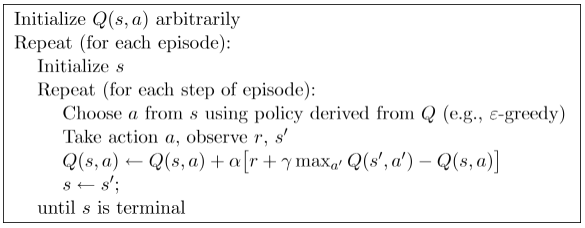
\includegraphics[scale=0.4]{./tex/reinforcement-learning/algo_Q-learning.png}
    \caption{Algorithme du Q-Learning(0)}
    \label{qalgo}
\end{figure}

\paragraph{Approximation des valeurs d'états}
Jusqu'ici, nous avons étudié des méthodes qui reposent sur un nombre de visites important d'un même  état\footnote{la convergence "parfaite" vers $V^*$ et $Q^*$ demande une visite infinie de chaque état par exemple...}. Cette condition n'est pas tenable en cas d'espace d'états de très grande dimension (ou infini) car les capacités calculatoires ne le permettent pas. Une approche consiste donc à ne plus évaluer chaque valeur d'état possibles mais à approximer une fonction capable de prédire n'importe quel état. Cette approche est très puissante car elle permet de prédire n'importe quel état, y compris des états jamais visités. Pour réaliser cela, il est nécessaire d'exploiter une méthode capable d'approximer des fonctions. Il est reconnu que les réseaux de neurones brillent dans cette tâche d'où leurs utilisations.\\

\noindent L'idée est simple. Un réseau reçoit une entrée associée à un état et la sortie du réseau produit une estimation de la valeur de cet état. En général, un état est caractérisé par différents attributs représentant l'entrée du réseau. Par exemple, dans le cas d'une voiture qui roule, on peut supposer les caractéristiques associées à la vitesse, l'état de la voiture, l'état de la route etc... Le réseau produit ainsi une valeur $\hat{V}(s)=f(s,\theta)$ (ou $\hat{Q}(s)$) avec $\theta$, poids du réseau (paramètres) qui pondèrent les caractéristiques de l'état observé. L'objectif du réseau est donc de minimiser l'erreur $||f(s,\theta)-V^*(s)||$ en trouvant la combinaison $\theta^*$ optimale. L'utilisation des réseaux de neurones soulèvent de nombreuses problématiques notamment l'apprentissage \textit{online} du réseau, l'exploitation de différences temporelles et non d'une valeur labellisée au pouvoir explicatif juste et nette. Il existe de nombreuses approches qui dépassent le cadre de ce cours mais qu'il est important de considérer si vous voulez pleinement maîtriser ce domaine.

\subsection{Deep Q-Learning}
Avec l'avènement du Deep Learning, les algorithmes de renforcement repose de plus en plus sur des structures neuronales. Dans le cadre de ce cours, nous exploiterons l'application des réseaux convolutifs pour la création de \textit{bots} pour des jeux vidéos de type \textit{ATARI}\footnote{Atari est une entreprise française (initialement américaine) de jeu vidéo fondée en 1972}. Ce n'est qu'un cas particulier de ce qui est possible de réaliser. Ce cours ne fournit qu'une sensibilisation à ce domaine à travers cet exemple mais un travail de recherche personnel sera nécessaire pour réaliser un état de l'art complet.\\

\noindent Un jeu, en apparence simple, peut présenter une complexité sous-jacente notamment liée aux différentes possibilités d'action réalisable dans le cadre d'une partie. Par exemple, le nombre de Shannon, $10^{120}$, est une estimation de la complexité du jeu d'échecs, c'est-à-dire du nombre de parties différentes réalisables dans le cadre d'une partie standard\footnote{Ce nombre est à dissocier du nombre total de partie réalisable qui est nettement plus élevé}. Les approches standards de l'apprentissage par renforcement reposent sur un apprentissage itératif basé sur une visite de nombreuses fois d'un même état de l'environnement. Il est évident qu'étant donné la dimension massive de l'espace d'états, ces approches ne sont pas humainement réalisables. Il est donc nécessaire d'étudier une approche plus généraliste capable d'étudier des problèmes à haute dimension.\\

\noindent Le Deep Q-learning\cite{dqn} exploite les capacités des réseaux neuronaux pour obtenir une approximation de la fonction Q qui définit la valeur de Q(s,a) dans un état s réalisant l'action a. Le réseau neuronal est ainsi capable d'évaluer chaque valeur Q(s,a) même si l'état s est peu ou pas visité (de même pour l'action réalisable dans cet état). Cette approche permet donc de résoudre la problématique de l'espace d'états à haute dimension.\\

\noindent Un robot-joueur possède les mêmes informations qu'un joueur humain. Ainsi, dans le cadre d'un jeu Atari, les informations à disposition sont les images de jeu \footnote{Dans le cadre d'autres jeux, comme le Cartpod par exemple, l'information à disposition peut être présentée sous forme de données numériques telles que la vitesse, l'angle par rapport à la verticale etc...}(en plus des récompenses associées à l'environnement telles que l'impact sur le score par exemple). Il est donc nécessaire d'adapter le réseau de neurones à cette spécificité d'où l'utilisation d'un réseau convolutif qui présente de bons résultats en analyse d'image.\\

\noindent Les données d'apprentissage du réseau correspondent à des tuples de données de la forme $<s_t,a_t,r_t,s_{t+1}>$ où $s_t$ correspond à un ensemble de N images successives (N=4 dans le cadre des jeux Atari), $a_t$ est l'action réalisée dans l'état $s_t$, $r_t$ est la récompense obtenue et $s_{t+1}$, l'état de l'automate après son action représenté par N images. Ces tuples présentent deux risques majeures. Le premier est la corrélation entre les données. Il est évident que l'image à l'instant t est liée à l'image à l'instant t+1 car c'est dans la continuité du jeu. Le second correspond à la distribution du jeu de données. Supposons le jeu du casse-briques, il est possible que l'automate, du fait de son initialisation aléatoire, favorise un des deux côtés de l'écran. Ceci est problématique car si non traitée, cette particularité peut inhiber l'exploitation d'une zone complète du jeu en favorisant le sur-apprentissage du réseau convolutif. Il est donc nécessaire de lutter contre la corrélation du jeu d'apprentissage et de permettre qu'il soit le plus représentatif de la distribution réelle du jeu observé.\\

\noindent Ces tuples sont obtenus au cours des expériences finies du jeu et sont conservés au sein du \textit{replay memory}, jeu d'apprentissage de K tuples où K élevé pour limiter les variations de distribution du jeu d'apprentissage associées aux expériences possiblement très variées de l'automate vis-à-vis du jeu. L'idée est que le comportement aléatoire initial de l'automate va permettre une exploration satisfaisante et la dimension élevée du jeu d'apprentissage permettra de limiter le risque de sur-spécialisation des images conservées. L'apprentissage du réseau de neurones sera réalisé avec un minibatch de k tuples tirés au hasard dans le \textit{replay memory} afin de limiter la corrélation entre les tuples qui est dangereuse pour l'apprentissage du réseau. Cette approche constitue l'\textit{Experience Replay}.\\

\noindent Dans le cadre du Q-learning, nous pouvons définir: $$Q_{i+1}(s_t,a_t)=E[r_t+\gamma*max_{a_{t+1}\in A_{s_{t+1}}}Q_i(s_{t+1},a_{t+1})|s_t,a_t]$$
Ainsi, l'objectif du réseau est d'approximer une fonction qui, pour tout s et a, minimise la fonction de perte suivante (de type \textit{Squared Error Loss}):
$$Loss=\frac{1}{2}.[\underbrace{r_t+\gamma* max_{a_{t+1}}(Q(s_{t+1},a_{t+1};\theta))}_\text{target}-\underbrace{Q(s_t,a_t;\theta)}_\text{prediction}]^2$$

\noindent L'architecture du réseau est visible sur la Figure \ref{deepql}. Cette architecture souffre des limitations théoriques des réseaux de neurones. Ainsi, il n'y a pas de convergence théorique démontrée bien qu'empiriquement stable. De plus, la distribution des scores de l'automate sont très bruitées et témoignent d'une variance importante. Cette variance témoigne du manque de robustesse du modèle qui présente une trop grande sensibilité aux variations des observations. De plus, on peut noter qu'une variation de faible ampleur des poids du réseau agit de manière significative sur les performances de l'automate (en bien comme en mal). Néanmoins, l'évolution des Q-values tend à converger. Cette dernière observation est contestable car la diminution des taux d'apprentissage simule ce comportement sans véritablement corriger les risques de divergence réels. Ca soigne les symptômes sans s'attaquer aux causes en quelque sorte... Néanmoins, les performances du modèle dépasse ses concurrents (de l'époque !) et dépasse parfois, l'homme lui-même. Cet algorithme présente, cependant, une faiblesse sur des jeux qui demandent une stratégie à long terme. La notion de mémoire est donc à améliorer sur cette algorithme.

\begin{figure}
    \centering
    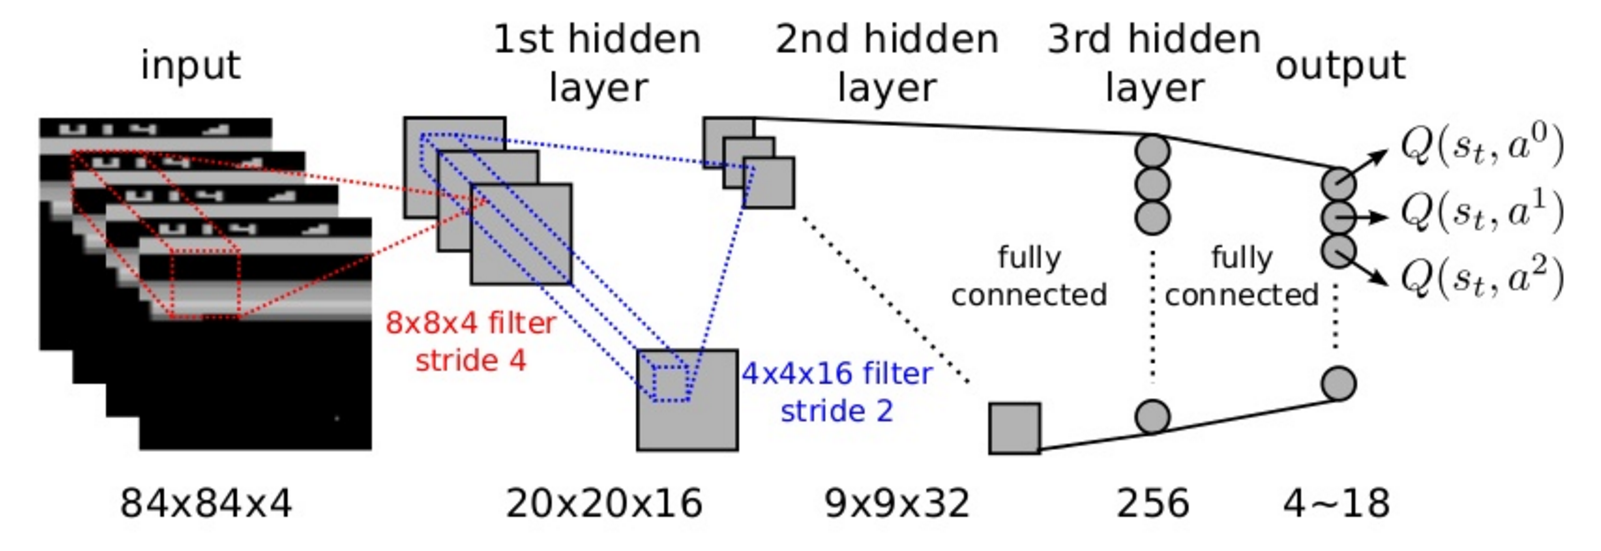
\includegraphics[scale=0.2]{./tex/reinforcement-learning/deepql.png}
    \caption{Algorithme du Deep Q-Learning}
    \label{deepql}
\end{figure}

\subsection{Prioritized Experience Replay}
Cette approche propose un postulat où des expériences sont porteuses de plus d'informations que d'autres. La sélection des expériences stockées dans l'Experience Replay étant aléatoire, il est probable que les expériences "riches" pour l'apprentissage se voient noyées dans l'ensemble des expériences pour la majorité peu riches. Afin de contrer ce problème, Prioritized Experience Replay\cite{priorexprep} propose une approche pour pondérer les expériences afin d'exploiter au mieux les expériences porteuses d'informations.\\

\noindent Pour juger de la pertinence d'une expérience, un indice de priorité est proposé. Il est défini par: $p_i=|\delta_i|+\epsilon$ avec i, index de l'i-ième expériences, $\delta$, erreur entre la prédiction réalisée par le modèle et la valeur effective à obtenir et $\epsilon$, constante non nulle pour éviter qu'une expérience ait un indice de priorité nul.\\

\noindent Utiliser une approche \textit{greedy} sur les indices de priorité (sélectionner que les expériences avec un fort indice) va imposer une sur-représentation de certaines expériences au détriment d'autres et de ce fait, favoriser l'overfitting du modèle. Pour limiter ce phénomène, un compromis entre une approche \textit{greedy} et une sélection aléatoire est nécessaire. L'approche \textit{Softmax} a donc été choisie pour réaliser ce compromis. Ainsi, à chaque expérience, nous associons une probabilité d'être sélectionnée $P_i$ définie telle que $P_i=\frac{p_i^\alpha}{\sum_kp_k^\alpha}$ avec $p_i$, indice de priorité de l'expérience i, k, nombre d'expériences et $\alpha$, constante qui définie l'importance de l'indice dans la détermination de la probabilité de sélection. Si $\alpha$ est égale à 0, nous obtenons une sélection aléatoire et si $\alpha \rightarrow \infty$, la sélection est \textit{greedy}.\\

\noindent Afin de limiter l'impact des \textit{outliers} (une expérience avec une erreur significativement plus grande que les autres)\footnote{Supposons un cas extrême où une expérience est infiniment plus grande que les autres. Cette expérience aura une probabilité quasi absolue d'être sélectionnée à chaque fois.}, il peut être nécessaire d'utiliser une autre métrique pour calculer l'indice de priorité. Ainsi, au lieu d'exploiter l'erreur de prédiction, l'indice reposera sur le \textit{rang} de cette erreur. Ainsi, l'erreur la plus importante aura un rang de 1 et l'erreur la moins importante, un rang de k (en supposant k expériences). L'indice de priorité est donc défini par: $\frac{1}{rank(i)}$. Cette approche tend à être plus robuste grâce à son insensibilité aux outliers mais les deux favorisent une vitesse de convergence significativement plus forte qu'avec une approche aléatoire.\\

\noindent Prioritized Experience Replay introduit un biais du fait de sa sélection non aléatoire. La sélection prioritaire de certaines expériences va forcer le modèle à apprendre de nombreuses fois sur un sous-ensemble d'expériences alors que d'autres seront peu ou pas examinées. Ce phénomène risque de provoquer un overfitting important à terme. Afin de corriger cette faiblesse, il est nécessaire de limiter l'impact d'une expérience souvent exploitée.\\

\noindent Pour cela, la valeur de l'erreur du modèle associée à l'expérience i est redéfinie par $w_i\delta_i$ avec $w_i=(\frac{1}{N}*\frac{1}{P_i})^\beta$ où N, taille du batch d'apprentissage du modèle et $\beta$, facteur d'importance permettant de définir l'impact de la régulation sur l'erreur produite par l'expérience. Une expérience souvent observée aura donc une influence régulière dans l'apprentissage du modèle mais son impact sera plus faible que celle des expériences plus rarement exploitées. Au début de l'apprentissage, on exploite une valeur de $\beta$ proche de 0 car, à cette étape, la présence d'un biais n'est pas trop impactant. Lorsque le modèle commence à converger, réguler le biais est nécessaire et de ce fait, la valeur de $\beta$ doit tendre vers 1. Ainsi, il sera pertinent, durant l'apprentissage, de faire varier continuellement $\beta$ de 0 vers 1 afin d'exploiter le pouvoir de converge d'une approche \textit{greedy} et la protection contre l'overfitting d'une approche stochastique.

\subsection{Double Deep Q-Learning}
\noindent  Dans l'algorithme du Q-Learning, l'opérateur max utilise la même valeur pour choisir une action et l'évaluer. Cette particularité va favoriser la sélection de valeurs surestimées suite à un excès d'optimisme dû aux erreurs d'apprentissage. En effet, supposons un état où chaque Q doit avoir une valeur identique lors d'une convergence idéale du modèle. Durant l'apprentissage, la présence de l'opérateur max dans l'algorithme du Q-Learning va introduire un biais associé aux valeurs de Q encore bruitées selon les expériences de l'apprentissage. En effet, la valeur de Q avec la plus grande erreur positive sera sélectionnée. Ce phénomène est appelé \textit{Overoptimism}. L'idée du Double Deep Q learning (DDQN)\cite{ddqn} est d'exploiter deux réseaux distincts pour évaluer une action et choisir l'action à réaliser. Cette approche permet ainsi de limiter l'optimisme de l'algorithme et d'être plus "modéré" sur les changements de comportements en limitant le biais de prédiction de $max_a$(Q(s,a,w)). Cette approche est très utile en début d'apprentissage car le manque d'informations fausse la pertinence des valeurs de Q. \\

\noindent Supposons deux réseaux dont l'ensemble des poids est représenté par $w_1$ et $w_2$. L'estimation de l'erreur par le DDQN devient donc:\\
$$Loss=\frac{1}{2}.(r_t+\gamma Q(s_{t+1},\textcolor{red}{argmax_{a_{t+1}}Q(s_{t+1},a_{t+1},w_1)},w_2)-Q(s_t,a_t;w_1))^2$$

\noindent Les deux modèles sont appris indépendamment et le réseau mis à jour choisi aléatoirement. Il est possible d'alterner le réseau qui prédit l'action à réaliser et sa valeur pour un apprentissage symétrique.\\

\noindent Pour des raisons de temps d'apprentissage et de coût matériel, cette approche n'est pas exploitée comme présentée précédemment. Une méthode subsidiaire permet de profiter de la majorité des bénéfices de l'approche \textit{Double} tout en limitant les exigences de calculs. Pour cela, le second modèle n'est pas complètement dissocié du premier mais est équivalent à une copie du modèle initial dont les poids correspondent aux poids du modèle initial à un instant t-n. La prédiction de la valeur de Q sera réalisée avec le modèle ancien et la prédiction de l'action à réaliser, par le réseau à jour. Cette particularité permet de s'émanciper d'un double apprentissage qui est gourmand en ressources matérielles et temporelles en se limitant à l'apprentissage d'un unique réseau.\\

\noindent Supposons 2 Q-network: un "à jour" (w), un "ancien" ($w^-$). (w) sélectionne l'action à réaliser et (w-) évalue la valeur de l'action. L'apprentissage du réseau suit la relation suivante:
$$Loss=\frac{1}{2}.(r_t+\gamma Q(s_{t+1},\textcolor{red}{argmax_{a_{t+1}}Q(s_{t+1},a_{t+1},w)},w^-)-Q(s_t,a_t;w))^2$$

\subsection{Dueling Deep Q-Learning}
\noindent Le modèle Dueling (DDQN)\cite{dudqn} repose sur l'idée que la valeur de Q est une combinaison de deux fonctions: A(a,s) qui représente la pertinence de faire une action a dans un état s et V(s), la pertinence d'être dans un état S\footnote{Cette combinaison peut laisser penser à une approche model-based qui vise à étudier les spécificités de l'environnement}. Cette séparation permet de considérer la qualité d'être dans un état indépendamment d'une action. Elle permet ainsi de mieux évaluer un état en l'émancipant d'une action associée. En effet, la plupart du temps, la valeur associée à la réalisation d'une action dans un état s n'a pas d'influence significative sur la valeur de l'état s. Pour considérer cette particularité, V et A sont calculées à partir de deux réseaux feed-forward issus d'une même source (couche de convolution ou un autre réseau feed-forward) et parfaitement isolés l'un de l'autre. Leurs sorties sont par la suite additionnées pour produire la valeur de Q.\\

\noindent Nous avons donc:
$$Q(s,a) = V(s) + A(s,a)$$
$$V(s)=E(Q(s,a))$$
$$A(s,a)=Q(s,a)-E(Q(s,a))$$
$$E(A(s,a))=0$$
$$Q(s,a)=V(s) \ and \ A(s,a)=0 \ if \ deterministic \ policy$$\\

\noindent Dans les faits, nous exploitons une valeur de A normalisée pour l'apprentissage soit:
$$Q(s,a,\theta,\alpha,\beta)=V(s,\theta,\beta)+(A(s,a,\theta,\alpha)-\frac{1}{|\mathcal{A}|}\sum_{a \in \mathcal{A}}A(s,a,\theta, \alpha)) $$
\noindent Cette régularisation permet d'assurer que l'un des flux du réseau Dueling déterminera bien la valeur d'un état. Il est aussi possible de régulariser par la valeur max de $A(s,a,\theta,\alpha)$ mais l'utilisation de la moyenne présente de meilleurs résultats. \\

\noindent Le réseau est illustré sur la Figure \ref{dudeepql}. Expérimentalement, il présente de meilleurs résultats que le DQN et le DDQN.
\begin{figure}
    \centering
    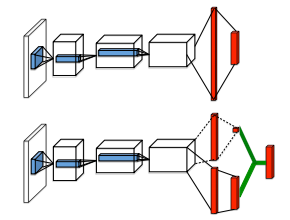
\includegraphics[scale=0.4]{./tex/reinforcement-learning/duelingdeepq.png}
    \caption{Algorithme du Dueling Deep Q-Learning}
    \label{dudeepql}
\end{figure}


\subsection{Double Dueling Q-Learning}
Le modèle Double Dueling Q-Learning (D-DDQN) est une approche qui unit le Double Q-Learning et le Dueling Q-Learning. Ainsi, DDQN exploitera deux réseaux distincts pour réaliser la prédiction de la valeur de Q et de l'action à réaliser (approche Double) et, au sein de ces réseaux, la prédiction de la valeur d'état et de la pertinence d'une action sera dissociée (approche Dueling).\\

\noindent Son efficacité tend à dépasser l'approche Double ou Dueling seule en profitant des bénéfices des deux approches.
